\documentclass[tikz, crop, border = {2pt 2pt 2pt 2pt}]{standalone}

\usepackage{concmath-otf}
\usetikzlibrary{calc, angles, quotes, patterns}
\usetikzlibrary{decorations.pathreplacing, decorations.pathmorphing, calligraphy}

\begin{document}
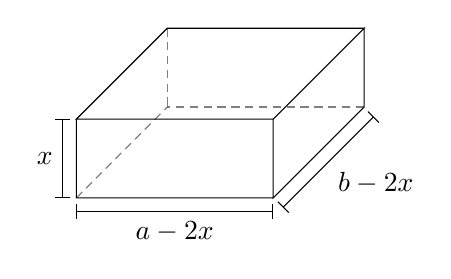
\begin{tikzpicture}
	\pgfmathsetmacro{\cubex}{2.5}
	\pgfmathsetmacro{\cubey}{1}
	\pgfmathsetmacro{\cubez}{3}
	\draw [draw=black, every edge/.append style = {densely dashed, opacity = .5}] (0, 0, 0) coordinate (o) -- ++ (-\cubex, 0, 0) coordinate (a) -- ++ (0, -\cubey, 0) coordinate (b) edge coordinate [pos = 1] (g) ++ (0, 0, -\cubez) -- ++(\cubex, 0, 0) coordinate (c) -- cycle
		(o) -- ++ (0, 0, -\cubez) coordinate (d) -- ++ (0, -\cubey, 0) coordinate (e) edge (g) -- (c) -- cycle
		(o) -- (a) -- ++ (0, 0, -\cubez) coordinate (f) edge (g) -- (d) -- cycle;
	\path [every edge/.append style = {|-|}]
		(b) + (0, -5pt) coordinate (b1) edge ["$a - 2x$"'] (b1 -| c)
		(b) + (-5pt, 0) coordinate (b2) edge ["$x$"] (b2 |- a)
		(c) + (3.5pt, -3.5pt) coordinate (c2) edge ["$b - 2x$"'] ([xshift = 3.5pt, yshift = -3.5pt]e);
\end{tikzpicture}
\end{document}
